\providecommand{\Fun}{\operatorname{Fun}}
\providecommand{\Cat}{\mathcal{C}at}
\providecommand{\sSet}{s\mathcal{S}et}
\providecommand{\QCat}{\mathcal{Q}\mathcal{C}at}
\providecommand{\qcOne}{\mathbf{1}}  %
\providecommand{\qcTwo}{\mathbf{2}}  %
\providecommand{\qcInt}{\mathbb{I}}  %
\providecommand{\rvEqArrow}{\mathrel{\stackrel{\sim}{\Rightarrow}}} %
\providecommand{\rvTfibArrow}{\mathrel{\stackrel{\sim}{\twoheadrightarrow}}} %
\providecommand{\hcat}[1]{\hbar #1}  %
\providecommand{\rvCorner}[1]{\ulcorner #1\urcorner} %
\providecommand{\hTwoCell}[5]{\tikz[baseline=-0.8ex]{%
  \node (rvl) at (0,0) {$#1$};
  \node (rvr) at (2.9,0) {$#2$};
  \draw[->] (rvl) to[bend left=28] node[above]{$\scriptstyle #3$} (rvr);
  \draw[->] (rvl) to[bend right=28] node[below]{$\scriptstyle #5$} (rvr);
  \node at (1.45,0) {$\scriptstyle #4$};}}

\section{\trHomotopyTwoCategory}\label{sec:homotopy-2-category}

小 1-\trCategory{}作为对象构成一个由\trCategory{}、\trFunctor{}与\trNaturalTransformation{}组成的%
严格的\textbf{2-\trCategory}（2-category）\footnote{附录 B 介绍 2-\trCategory{}与 2-\trFunctor{}，
综述此处所需的 2-范畴论。简言之，与题外话 1.2.4 相平行地，%
2-\trCategory{}（见附录 B 中的\cref{def:two-category}）
可以同等地理解为：「二维」的\trCategory——有对象；1-\trCell{}，其边缘由一对对象给出；
以及 2-\trCell{}，其边缘由一对对象之间的一对平行 1-\trCell{}给出——连同由这份边缘数据
支配的、部分定义的复合操作；或者理解为富集于 $\Cat$ 之上的\trCategory{}。} $\Cat$。
许多基本的范畴论概念——即那些借助\trCategory{}、\trFunctor{}与\trNaturalTransformation{}%
定义的概念——都可以在 2-\trCategory $\Cat$ 内部定义。这暗示出一条自然的推广途径：
在一般的 2-\trCategory{}中重新解释这些同样的定义——用其对象代替小\trCategory{}，
用其\textbf{1-\trCell}（1-cell）代替\trFunctor{}，
用其\textbf{2-\trCell}（2-cell）代替\trNaturalTransformation{}。

在第 2 章中，我们将完全按照这一提纲，在任意取定的一个\trInfinityCosmos{}内部
发展\trInfinityCategory{}理论的相当大一部分：我们将在一座 2-\trCategory{}之中工作，
这座 2-\trCategory{}就是我们配属于任何\trInfinityCosmos{}的\emph{\trHomotopyTwoCategory}。
\trInfinityCosmos{}的\trHomotopyTwoCategory{}是整个\trInfinityCosmos{}的一个商：
把每个\trQuasiCategory{}性的\trFunctorSpace{}换成它的\trHomotopyCategory{}。令人惊讶的是，
这一颇具破坏性的取商操作竟保住了相当多的信息。事实上，
第一部分中\trInfinityCategory{}理论的几乎全部发展都发生于某个\trInfinityCosmos{}的%
\trHomotopyTwoCategory{}之中。话虽如此，我们还是要告诫读者切勿过度迷恋\trHomotopyTwoCategory{}：
与其说它是\trInfinityCategory{}理论的一个基础性概念，
不如说它是降低论证复杂度的一种技术性便利。

\trQuasiCategory{}之\trInfinityCosmos{}的\trHomotopyTwoCategory{}由 Joyal 在其关于\trQuasiCategory{}理论基础的
著作中率先引入\cite{bib63}。

\begin{definition}[\trHomotopyTwoCategory]\label{def:homotopy-2-category}
设 $\mathcal{K}$ 为一个\trInfinityCosmos{}。它的%
\textbf{\trHomotopyTwoCategory}（homotopy 2-category）是如下的 2-\trCategory
$\hcat{\mathcal{K}}$：
\begin{itemize}
\item 对象是 $\mathcal{K}$ 的对象 $A$，$B$，亦即诸\trInfinityCategory{}；
\item 1-\trCell $f\colon A\to B$ 是\trFunctorSpace $\Fun(A,B)$ 中的 0-箭头，
  即诸∞-\trFunctor{}；
\item 2-\trCell \hTwoCell{A}{B}{f}{\Downarrow\alpha}{g}
  是 $\Fun(A,B)$ 中 1-单纯形的\trHomotopy{}类，
  我们称之为\textbf{∞-\trNaturalTransformation}（∞-natural transformation）。
\end{itemize}
\end{definition}

换一种说法：$\hcat{\mathcal{K}}$ 是与 $\mathcal{K}$ 具有相同对象的 2-\trCategory{}，
其 hom-\trCategory{}定义为
\begin{equation*}
\mathrm{h}\Fun(A,B)\coloneqq\mathrm{h}(\Fun(A,B)),
\end{equation*}
也就是说，$\mathrm{h}\Fun(A,B)$ 就是\trQuasiCategory $\Fun(A,B)$ 的\trHomotopyCategory{}。

一个 2-\trCategory{}的\textbf{底范畴}（underlying category）由简单地遗忘其 2-\trCell{}而定义。
注意\trInfinityCosmos{} $\mathcal{K}$ 与其\trHomotopyTwoCategory $\hcat{\mathcal{K}}$
共享同一个由 $\mathcal{K}$ 中的\trInfinityCategory{}与∞-\trFunctor{}构成的底范畴 $\mathcal{K}_0$。

\begin{digression}[\trChangeOfBase{}，附录 A.7]\label{dig:change-of-base}
\trHomotopyCategory\trFunctor{}保持有限积，其右\trAdjunction{}当然亦然。
于是，命题 1.1.11 的\trAdjunction{}诱导出一个\trChangeOfBase\trAdjunction
\begin{center}
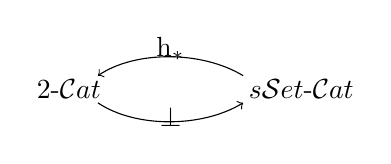
\begin{tikzpicture}[x=1.5em,y=1.4em]
  \node (l) at (0,0) {$2$-$\Cat$};
  \node (r) at (5.6,0) {$\sSet$-$\Cat$};
  \draw[->] (4.2,0.35) .. controls (3.2,1.0) and (1.6,1.0) .. (0.7,0.35);
  \node at (2.45,1.05) {$\mathrm{h}_*$};
  \draw[->] (0.7,-0.35) .. controls (1.6,-1.0) and (3.2,-1.0) .. (4.2,-0.35);
  \node at (2.45,-0.72) {$\perp$};
\end{tikzpicture}
\end{center}
其左、右\trAdjunction{}通过把\trHomotopyCategory\trFunctor{}或\trNerve\trFunctor{}应用于%
\trEnrichedCategory{}的 hom 对象来变更富集。这里 $2$-$\Cat$ 与 $\sSet$-$\Cat$
各自都可以理解为 2-\trCategory——由\trEnrichedCategory{}、富集\trFunctor{}与富集%
\trNaturalTransformation{}构成——并且这两个\trChangeOfBase{}构造都定义 2-\trFunctor
（见命题 A.7.3 与 A.7.5）。%
由于\trNerve{}嵌入是\trFullyFaithful，2-\trCategory{}可以等同于一个满子\trCategory{}，
由那些 hom 空间皆为\trCategory{}之\trNerve{}的\trSimplicialCategory{}组成。
\end{digression}

引理 1.3.12 的证明用到了一个值得单独点出的观察：%
\begin{lemma}\label{lem:represent-2-cells}
(i) \trInfinityCosmos{}的\trHomotopyTwoCategory{}中的每个 2-\trCell
\hTwoCell{A}{B}{f}{\Downarrow\alpha}{g}
都由一个如下左图所示的\trQuasiCategory{}映射表示，或\trEquivalence{}地，由一个如下右图所示的%
\trFunctor{}表示
\begin{center}
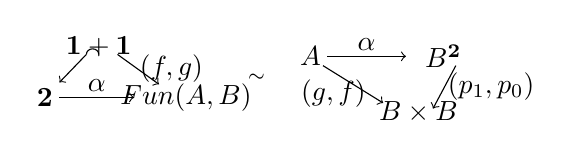
\begin{tikzpicture}[x=1.5em,y=1.35em]
  \node (fg) at (1.3,1.35) {$\qcOne+\qcOne$};
  \node (two) at (0,0) {$\qcTwo$};
  \node (fun) at (3.4,0) {$\Fun(A,B)$};
  \draw[->] (1.0,1.15) -- (0.35,0.4);
  \draw (1.0,1.15) arc[start angle=180,end angle=0,radius=0.15];
  \draw[->] (1.75,1.15) -- (2.75,0.35);
  \node at (3.05,0.78) {$(f,g)$};
  \draw[->] (0.35,0) -- (2.15,0);
  \node at (1.25,0.32) {$\alpha$};
  \node at (5.1,0.5) {$\stackrel{\sim}{\leftrightharpoons}$};
  \begin{scope}[shift={(6.4,0)}]
    \node (A) at (0,1.1) {$A$};
    \node (B2) at (3.2,1.1) {$B^{\qcTwo}$};
    \node (BB) at (2.6,-0.4) {$B\times B$};
    \draw[->] (0.4,1.1) -- (2.3,1.1);
    \node at (1.35,1.42) {$\rvCorner{\alpha}$};
    \draw[->] (0.3,0.85) -- (1.75,-0.15);
    \node at (0.55,0.1) {$(g,f)$};
    \draw[->] (3.5,0.85) -- (2.95,-0.3);
    \node at (4.35,0.3) {$(p_1,p_0)$};
  \end{scope}
\end{tikzpicture}
\end{center}
并且两个这样的映射表示同一个 2-\trCell{}，当且仅当它们作为 $\Fun(A,B)$ 中的
1-单纯形是\trHomotopy{}的。
(ii) \trInfinityCosmos{}的\trHomotopyTwoCategory{}中的每个可逆 2-\trCell
\hTwoCell{A}{B}{f}{\cong\;\Downarrow\alpha}{g}
都由一个如下左图所示的\trQuasiCategory{}映射表示，或\trEquivalence{}地，由一个如下右图所示的%
\trFunctor{}表示
\begin{center}
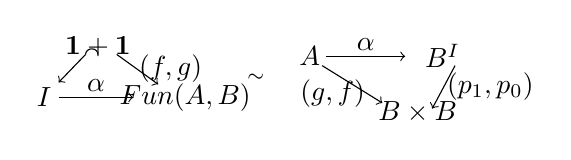
\begin{tikzpicture}[x=1.5em,y=1.35em]
  \node (fg) at (1.3,1.35) {$\qcOne+\qcOne$};
  \node (two) at (0,0) {$\qcInt$};
  \node (fun) at (3.4,0) {$\Fun(A,B)$};
  \draw[->] (1.0,1.15) -- (0.35,0.4);
  \draw (1.0,1.15) arc[start angle=180,end angle=0,radius=0.15];
  \draw[->] (1.75,1.15) -- (2.75,0.35);
  \node at (3.05,0.78) {$(f,g)$};
  \draw[->] (0.35,0) -- (2.15,0);
  \node at (1.25,0.32) {$\alpha$};
  \node at (5.1,0.5) {$\stackrel{\sim}{\leftrightharpoons}$};
  \begin{scope}[shift={(6.4,0)}]
    \node (A) at (0,1.1) {$A$};
    \node (BI) at (3.2,1.1) {$B^{\qcInt}$};
    \node (BB) at (2.6,-0.4) {$B\times B$};
    \draw[->] (0.4,1.1) -- (2.3,1.1);
    \node at (1.35,1.42) {$\rvCorner{\alpha}$};
    \draw[->] (0.3,0.85) -- (1.75,-0.15);
    \node at (0.55,0.1) {$(g,f)$};
    \draw[->] (3.5,0.85) -- (2.95,-0.3);
    \node at (4.35,0.3) {$(p_1,p_0)$};
  \end{scope}
\end{tikzpicture}
\end{center}
并且两个这样的映射表示同一个可逆 2-\trCell{}，当且仅当它们沿
$\qcTwo\hookrightarrow\qcInt$ 的公共限制作为 $\Fun(A,B)$ 中的 1-单纯形是\trHomotopy{}的。
\end{lemma}

此处引用的「\trHomotopy{}的 1-单纯形」概念定义于引理 1.1.9。
由于\trHomotopyTwoCategory{}中的 2-\trCell{}被称为∞-\trNaturalTransformation{}，
我们把\trHomotopyTwoCategory{}中的可逆 2-\trCell{}称作\textbf{\trInfinityNaturalIsomorphism}
（∞-natural isomorphism）。

\begin{proof}
陈述 (i) 记录了\trHomotopyTwoCategory{}中 2-\trCell{}的定义以及单纯\trCotensor{}的泛性质 (1.2.7)。
对于 (ii)，\trHomotopyTwoCategory{}中的一个 2-\trCell{}是\textbf{可逆的}，
当且仅当它在相应的 hom-\trCategory $\mathrm{h}\Fun(A,B)$ 中定义一个\trIsomorphism{}。
由推论 1.1.16，%
每个可逆 2-\trCell $\alpha$ 都由一个\trHomotopyCoherentIsomorphism
$\alpha\colon\qcInt\to\Fun(A,B)$ 表示，
后者类似地内化而定义一个\trFunctor{} $\rvCorner{\alpha}\colon A\to B^{\qcInt}$。
\end{proof}

\cref{dig:change-of-base} 的一个附带结论是：\trChangeOfBase{}这一操作不仅适用于\trEnrichedCategory{}，
也适用于富集\trFunctor——在最令人感兴趣的情形中，这可以直接验证。
\begin{lemma}\label{lem:simplicial-functor-2-functor}
\trInfinityCosmos{}之间的任何单纯\trFunctor{} $F\colon\mathcal{K}\to\mathcal{L}$
都诱导其\trHomotopyTwoCategory{}之间的一个 2-\trFunctor
$F\colon\hcat{\mathcal{K}}\to\hcat{\mathcal{L}}$。
\end{lemma}
\begin{proof}
诱导的 2-\trFunctor $F\colon\hcat{\mathcal{K}}\to\hcat{\mathcal{L}}$
在对象与 1-\trCell{}上的作用由 $F\colon\mathcal{K}\to\mathcal{L}$ 的相应作用给出；
回忆\trInfinityCosmos{}与其\trHomotopyTwoCategory{}具有相同的底 1-\trCategory{}。
$\hcat{\mathcal{K}}$ 中的每个 2-\trCell{}都由 $\Fun(A,B)$ 中的一个 1-单纯形表示，
后者经由
\begin{equation*}
\begin{array}{c}
\Fun(A,B)\xrightarrow{\;F\;}\Fun(FA,FB)\\[8pt]
\hTwoCell{A}{B}{f}{\Downarrow\alpha}{g}\\[8pt]
\;\longmapsto\;\hTwoCell{FA}{FB}{Ff}{\Downarrow F\alpha}{Fg}
\end{array}
\end{equation*}
被送到 $\hcat{\mathcal{L}}$ 中表示某个 2-\trCell{}的一个 1-单纯形。
由于作用\trFunctor $F\colon\Fun(A,B)\to\Fun(FA,FB)$
定义\trSimplicialSet{}之间的映射，它保持面与退化。特别地，
$\Fun(A,B)$ 中\trHomotopy{}的 1-单纯形被送到 $\Fun(FA,FB)$ 中\trHomotopy{}的 1-单纯形，
故刚才描述的 2-\trCell{}上的作用是良定义的。
而这些映射的 2-\trFunctor{}性则从原来那个映射的\trSimplicialFunctor{}性得出。
\end{proof}

现在我们开始把一个\trInfinityCosmos{}的单纯富集结构与它的\trHomotopyTwoCategory{}中的
2-\trCategory{}结构联系起来：证明\trHomotopyTwoCategory{}从其\trInfinityCosmos{}那里继承了满足某种 2-\trCategory{}泛性质的
积。为作说明，回忆终\trInfinityCategory{} $1\in\mathcal{K}$ 具有泛性质
$\Fun(X,1)\cong 1$（对一切 $X\in\mathcal{K}$）。
应用\trHomotopyCategory\trFunctor{}可见 $1\in\hcat{\mathcal{K}}$ 具有泛性质
$\mathrm{h}\Fun(X,1)\cong 1$（对一切 $X\in\hcat{\mathcal{K}}$），
这就表述为：\trInfinityCategory $1$ 在\trHomotopyTwoCategory{}中定义一个\textbf{\trTwoTerminalObject}
（2-terminal object）。这条 2-\trCategory{}泛性质兼有 1 维面向与 2 维面向：
由于 $\mathrm{h}\Fun(X,1)\cong 1$ 是只有一个对象的\trCategory{}，
$\mathcal{K}$ 中存在唯一的态射 $X\to 1$；
又由于 $\mathrm{h}\Fun(X,1)\cong 1$ 只有一个态射，
$\hcat{\mathcal{K}}$ 中以 $1$ 为余域的 2-\trCell{}只有恒等者。

\begin{proposition}[笛卡尔封闭]\label{prop:cartesian-closure}
\begin{enumerate}[label=(\roman*)]
\item 任何\trInfinityCosmos{}的\trHomotopyTwoCategory{}都有 2-\trCategory{}的积。
\item \trCartesianClosed\trInfinityCosmos{}的\trHomotopyTwoCategory{}作为 2-\trCategory{}是%
\trCartesianClosed{}。
\end{enumerate}
\end{proposition}

\begin{proof}
\trFunctor $\mathrm{h}\colon\sSet\to\Cat$ 只保持有限积，
而受限\trFunctor $\mathrm{h}\colon\QCat\to\Cat$ 保持\emph{一切}积——
这归功于引理 1.1.12 所给的\trQuasiCategory{}\trHomotopyCategory{}之简化描述。
于是，对任何集合 $I$ 与 $\mathcal{K}$ 中的\trInfinityCategory{}族 $(A_i)_{i\in I}$，
\trHomotopyCategory\trFunctor{}把\trFunctorSpace{}的\trIsomorphism{}送到 hom-\trCategory{}的\trIsomorphism{}：
\begin{equation*}
\begin{array}{c}
\Fun\Bigl(X,\displaystyle\prod_{i\in I}A_i\Bigr)
\xrightarrow{\;\simeq\;}
\displaystyle\prod_{i\in I}\Fun(X,A_i)\\[8pt]
\downarrow\mathrm{h}\\[8pt]
\mathrm{h}\Fun\Bigl(X,\displaystyle\prod_{i\in I}A_i\Bigr)
\xrightarrow{\;\simeq\;}
\displaystyle\prod_{i\in I}\mathrm{h}\Fun(X,A_i).
\end{array}
\end{equation*}
这证明\trHomotopyTwoCategory $\hcat{\mathcal{K}}$ 有积，
其泛性质兼有 1 维与 2 维两种成分，
一如上文对终对象的空情形所作的描述。

若 $\mathcal{K}$ 是\trCartesianClosed\trInfinityCosmos{}，
则对任意三个\trInfinityCategory $A$，$B$，$C\in\mathcal{K}$，
存在指数对象 $C^A$ 与 $C^B\in\mathcal{K}$，
由自然\trIsomorphism{}刻画：
\begin{equation*}
\Fun(A\times B,C)\cong\Fun(A,C^B)\cong\Fun(B,C^A).
\end{equation*}
过渡到\trHomotopyCategory{}，便有自然\trIsomorphism
\begin{equation*}
\mathrm{h}\Fun(A\times B,C)\cong\mathrm{h}\Fun(A,C^B)\cong\mathrm{h}\Fun(B,C^A),
\end{equation*}
这表明 $\hcat{\mathcal{K}}$ 作为 2-\trCategory{}是\trCartesianClosed{}：
\trFunctor{} $A\times B\to C$ 经转置定义\trFunctor{} $A\to C^B$ 与
$B\to C^A$，而\trNaturalTransformation{}也类似地转置。
\end{proof}

在任何 1-\trCategory{}中，都有一对对象之间\emph{\trIsomorphism}的标准定义，
且它为任何\trFunctor{}所保持。类似地，在任何 2-\trCategory{}中，
都有一对对象之间\emph{\trEquivalence}的标准定义，且它为任何 2-\trFunctor{}所保持：

\begin{definition}[\trEquivalence]\label{def:equivalence-2-category}
2-\trCategory{}中的\textbf{\trEquivalence}（equivalence）由下列数据给出：
\begin{itemize}
\item 一对对象 $A$ 与 $B$；
\item 一对 1-\trCell $f\colon A\to B$ 与 $g\colon B\to A$；以及
\item 一对可逆 2-\trCell
\begin{center}
\hTwoCell{A}{A}{\mathrm{id}_A}{\cong\;\Downarrow\alpha}{gf}
\qquad\text{及}\qquad
\hTwoCell{B}{B}{fg}{\cong\;\Downarrow\beta}{\mathrm{id}_B}
\end{center}
\end{itemize}
当 $A$ 与 $B$ \textbf{\trEquivalence}时，记 $A\simeq B$，
并把 1-\trCell $f$ 与 $g$ 称作\textbf{\trEquivalence}，记作「$\Rightarrow$」。
\end{definition}

对于一个\trInfinityCosmos{}的\trHomotopyTwoCategory{}而言，我们另有来自 1.2.1 的一个
与之竞争的\trEquivalence{}定义：即一个在\trFunctorSpace{}上诱导\trEquivalence
$f_\ast\colon\Fun(X,A)\rvEqArrow\Fun(X,B)$ 的 1-\trCell
$f\colon A\rvEqArrow B$——或者\trEquivalence{}地，按引理 1.2.15，
一个相对区间 $\qcInt$ 定义的\emph{\trHomotopy\trEquivalence}。
关键的是，这三条\trEquivalence{}定义相互重合：

\begin{theorem}[\trEquivalence{}是\trEquivalence]\label{thm:equivalences-are-equivalences}
在任何\trInfinityCosmos{} $\mathcal{K}$ 中，下列诸条件\trEquivalence{}，
并且刻画了\trInfinityCategory{}之间的\trFunctor{} $f\colon A\to B$
何时定义一个\textbf{\trEquivalence}。
\begin{enumerate}[label=(\roman*)]
\item 对一切 $X\in\mathcal{K}$，\trPostComposition{}映射
  $f_\ast\colon\Fun(X,A)\rvEqArrow\Fun(X,B)$
  定义\trQuasiCategory{}的\trEquivalence{}。
\item 存在\trFunctor{} $g\colon B\to A$ 以及\trHomotopyTwoCategory{}中的自然\trIsomorphism
  $\alpha\colon\mathrm{id}_A\cong gf$ 与
  $\beta\colon fg\cong\mathrm{id}_B$。
\item 存在\trFunctor{} $g\colon B\to A$ 以及映射
\begin{center}
\begin{tikzpicture}[x=1.35em,y=1.05em]
  \node (lA) at (0,0) {$A$};
  \node (tA) at (2.2,1.3) {$A$};
  \node (Ai) at (2.2,0) {$A^{\qcInt}$};
  \node (bA) at (2.2,-1.3) {$A$};
  \draw[double] (lA) -- (tA);
  \draw[->] (Ai) -- (tA) node[midway,right]{$\mathrm{ev}_0$};
  \draw[->] (lA) -- (Ai) node[midway,above]{$\alpha$};
  \draw[->] (lA) -- (bA) node[midway,below]{$gf$};
  \draw[->] (Ai) -- (bA) node[midway,right]{$\mathrm{ev}_1$};
  \node at (4.1,0) {及};
  \node (lB) at (6,0) {$B$};
  \node (tB) at (8.2,1.3) {$B$};
  \node (Bi) at (8.2,0) {$B^{\qcInt}$};
  \node (bB) at (8.2,-1.3) {$B$};
  \draw[->] (lB) -- (tB) node[midway,above]{$fg$};
  \draw[->] (Bi) -- (tB) node[midway,right]{$\mathrm{ev}_0$};
  \draw[->] (lB) -- (Bi) node[midway,above]{$\beta$};
  \draw[double] (lB) -- (bB);
  \draw[->] (Bi) -- (bB) node[midway,right]{$\mathrm{ev}_1$};
\end{tikzpicture}
\end{center}
位于\trInfinityCosmos $\mathcal{K}$ 之中。
\end{enumerate}
\end{theorem}
作为一则示意性比较：我们不是援引引理 1.2.15 来证明 (i)$\Leftrightarrow$(iii)，
而是以 2-范畴论与拟范畴论的技术重新证明它。
\begin{proof}
(i)$\Rightarrow$(ii)：若诱导映射 $f_\ast\colon\Fun(X,A)\rvEqArrow\Fun(X,B)$
定义\trQuasiCategory{}的\trEquivalence{}，则\trFunctor
$f_\ast\colon\mathrm{h}\Fun(X,A)\to\mathrm{h}\Fun(X,B)$ 定义\trCategory{}的\trEquivalence{}，
见注 1.1.24。%
特别地，\trEquivalence{} $f_\ast\colon\mathrm{h}\Fun(B,A)\to\mathrm{h}\Fun(B,B)$
本质满，%
故存在 $g\in\mathrm{h}\Fun(B,A)$ 以及\trIsomorphism
$\beta\colon fg\cong\mathrm{id}_B\in\mathrm{h}\Fun(B,B)$。
又因 $f_\ast\colon\mathrm{h}\Fun(A,A)\to\mathrm{h}\Fun(A,B)$ 是\trFullyFaithful，
\trIsomorphism $\beta f\colon fgf\cong f\in\mathrm{h}\Fun(A,B)$
可被\trLifting{}以定义\trIsomorphism $\alpha^{-1}\colon gf\cong\mathrm{id}_A\in\mathrm{h}\Fun(A,A)$。
这就定义了\cref{def:equivalence-2-category} 中 2-\trCategory\trEquivalence{}的数据。

(ii)$\Rightarrow$(iii)：回忆\cref{lem:represent-2-cells}：
\trHomotopyTwoCategory{}中的自然\trIsomorphism $\alpha\colon\mathrm{id}_A\cong gf$ 与
$\beta\colon fg\cong\mathrm{id}_B$ 由 $\mathcal{K}$ 中的映射
$\alpha\colon A\to A^{\qcInt}$ 与 $\beta\colon B\to B^{\qcInt}$ 表示，
如 (1.2.16) 所示。%

最后，(iii)$\Rightarrow$(i)：因为 $\Fun(X,-)$ 把 (iii) 的数据变成定义 1.1.23
意义下\trQuasiCategory\trEquivalence{}的数据。
\end{proof}

\cref{thm:equivalences-are-equivalences} 对后续工作的重要性怎么强调都不为过。
我们为\trInfinityCategory{}、∞-\trFunctor{}与∞-\trNaturalTransformation{}引进的种种范畴论构造，
都在\trHomotopyTwoCategory{}中对 2-\trCategory{}的\trEquivalence{}不变，
而我们发展的诸泛性质同样刻画\trInfinityCategory{}的 2-\trCategory\trEquivalence{}类。
\cref{thm:equivalences-are-equivalences} 于是断言：这类构造是
「\trHomotopy{}式正确的」——既对\trInfinityCosmos{}中的\trEquivalence{}不变，
又精确地识别对象的\trEquivalence{}类。

\trFunctorSpace{}在余域变元处的\trEquivalence{}不变性是公理化的，
但在定义域变元处的\trEquivalence{}不变性则不是。%
\footnote{引理 1.3.2 不适用，因为 $\Fun(-,B)$ 不是宇宙论\trFunctor{}。}
从\cref{thm:equivalences-are-equivalences}的 (i) 或 (iii) 出发，
也看不出这一点如何能够被证明。但借助 (ii) 与 2-\trCategory{}技术，
现在有了一条简短的证明。

\begin{corollary}\label{cor:functor-space-equivalences}
\trInfinityCategory{}的\trEquivalence{} $A'\rvEqArrow A$ 与 $B\rvEqArrow B'$
诱导\trFunctorSpace{}的\trEquivalence{} $\Fun(A,B)\rvEqArrow\Fun(A',B')$。
\end{corollary}
\begin{proof}
可表示\trSimplicialFunctor $\Fun(A,-)\colon\mathcal{K}\to\QCat$ 与
$\Fun(-,B)\colon\mathcal{K}^{\mathrm{op}}\to\QCat$
诱导 2-\trFunctor $\Fun(A,-)\colon\hcat{\mathcal{K}}\to\hcat{\QCat}$ 与
$\Fun(-,B)\colon\hcat{\mathcal{K}^{\mathrm{op}}}\to\hcat{\QCat}$，
它们保持\cref{def:equivalence-2-category} 的 2-\trCategory\trEquivalence{}。
由\cref{thm:equivalences-are-equivalences}，这正是所要证明的。
\end{proof}

还有一种标准的 2-\trCategory{}式的\trIsofibration{}概念，
其定义见于\cref{prop:isofibrations-are-isofibrations} 的陈述，并在附录 B 中的%
\cref{def:rajri-isofibration}中得到细化。
我们现在证明：\trInfinityCosmos{}中的任何\trIsofibration{}%
都在其\trHomotopyTwoCategory{}中定义一个\trIsofibration{}。

\begin{proposition}[\trIsofibration{}是\trIsofibration]\label{prop:isofibrations-are-isofibrations}
\trInfinityCosmos{} $\mathcal{K}$ 中的\trIsofibration{}
$p\colon E\twoheadrightarrow B$ 也在\trHomotopyTwoCategory $\hcat{\mathcal{K}}$ 中
定义一个\textbf{\trIsofibration}：给定任何如下左图所示、贴合于 $B$
的可逆 2-\trCell{}，连同其一侧边缘 1-\trCell{}穿过 $p$ 的一个指定\trLifting{}，
则存在如下右图所示、贴合于 $E$ 且以这条边缘 1-\trCell{}为其边缘的
可逆 2-\trCell{}，它与 $p$ 作须状复合后给出原来的 2-\trCell{}。
\begin{center}
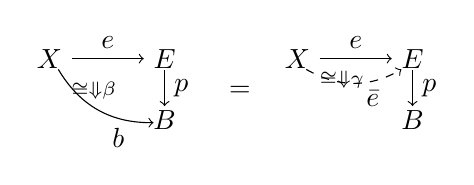
\begin{tikzpicture}[x=1.6em,y=1.3em]
  \node (X) at (0,1) {$X$};
  \node (E) at (2.6,1) {$E$};
  \node (B) at (2.6,-0.7) {$B$};
  \draw[->] (X) -- (E) node[midway,above]{$e$};
  \draw[->] (2.6,0.68) -- (2.6,-0.32) node[midway,right]{$p$};
  \draw[->] (0.2,0.7) to[bend right=30] node[pos=0.7,below]{$b$} (2.35,-0.78);
  \node at (1.0,0.12) {$\scriptstyle\cong\Downarrow\beta$};
  \node at (4.3,0.1) {$=$};
  \begin{scope}[shift={(5.6,0)}]
    \node (X2) at (0,1) {$X$};
    \node (E2) at (2.6,1) {$E$};
    \node (B2) at (2.6,-0.7) {$B$};
    \draw[->] (X2) -- (E2) node[midway,above]{$e$};
    \draw[->] (2.6,0.68) -- (2.6,-0.32) node[midway,right]{$p$};
    \draw[->,dashed] (0.2,0.7) to[bend right=30] node[pos=0.7,below]{$\bar{e}$} (2.35,0.7);
    \node at (1.0,0.42) {$\scriptstyle\cong\Downarrow\gamma$};
  \end{scope}
\end{tikzpicture}
\end{center}
\end{proposition}
\begin{proof}
所述的泛性质说：\trFunctor
\begin{equation*}
p_\ast\colon\mathrm{h}\Fun(X,E)\rvTfibArrow\mathrm{h}\Fun(X,B)
\end{equation*}
是命题 1.2.11 所定义意义下\trCategory{}的\trIsofibration{}。
由\cref{def:infinity-cosmos}(ii)，
由于 $p\colon E\twoheadrightarrow B$ 是 $\mathcal{K}$ 中的\trIsofibration{}，
诱导映射 $p_\ast\colon\Fun(X,E)\twoheadrightarrow\Fun(X,B)$
是\trQuasiCategory{}的\trIsofibration{}。于是只需证明：
\trFunctor $\mathrm{h}\colon\QCat\to\Cat$
把\trQuasiCategory{}的\trIsofibration{}变为\trCategory{}的\trIsofibration{}。

那么现在考虑\trQuasiCategory{}之间的一个\trIsofibration{} $p\colon E\twoheadrightarrow B$。
由推论 1.1.16，%
\trQuasiCategory $B$ 的\trHomotopyCategory $\mathrm{h}B$ 中的每个\trIsomorphism $\beta$
都由一个\trSimplicialMap{} $\beta\colon\qcInt\to B$ 表示。
按定义 1.1.17，%
\trLifting{}问题
\begin{center}
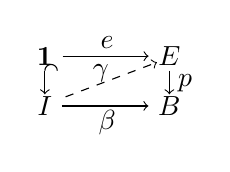
\begin{tikzpicture}[x=1.5em,y=1.5em]
  \node (tl) at (0,1.2) {$\qcOne$};
  \node (tr) at (3.0,1.2) {$E$};
  \node (bl) at (0,0) {$\qcInt$};
  \node (br) at (3.0,0) {$B$};
  \draw[->] (tl) -- (tr);
  \node at (1.5,1.52) {$e$};
  \draw[->] (0,0.85) -- (0,0.28);
  \draw (0,0.85) arc[start angle=180,end angle=0,radius=0.15];
  \draw[->,dashed] (0.5,0.22) -- (2.7,1.05);
  \node at (1.35,0.78) {$\gamma$};
  \draw[->] (3.0,0.85) -- (3.0,0.28);
  \node at (3.38,0.55) {$p$};
  \draw[->] (bl) -- (br);
  \node at (1.5,-0.4) {$\beta$};
\end{tikzpicture}
\end{center}
可解，而且这样得出的映射 $\gamma\colon\qcInt\to E$ 表示：
把该\trIsomorphism{}从 $\mathrm{h}B$ \trLifting{}为 $\mathrm{h}E$ 中以 $e$ 为定义域的\trIsomorphism{}。
\end{proof}

\begin{convention}[\trHomotopyTwoCategory{}中的\trIsofibration]\label{conv:isofibration-homotopy-2-category}
由于\cref{prop:isofibrations-are-isofibrations}的逆命题不成立，
用「\trIsofibration」一词指称\trInfinityCosmos{}的\trHomotopyTwoCategory{}中的映射时，
存在潜在的歧义。我们采取如下约定：当我们宣称 $\hcat{\mathcal{K}}$
中的一个映射是\trIsofibration{}时，指的总是较强的意义，
即在 $\mathcal{K}$ 中定义一个\trIsofibration{}。
这一较强条件使我们既能享有\cref{prop:isofibrations-are-isofibrations}的
2-\trCategory{}提升性质，又能享有定义 1.2.1 所公理化的\trHomotopy{}论性质，
后者保证 1.2.1(i) 中严格定义的\trLimit{}自动是\trEquivalence{}不变的构造
（见附录 C.1 与命题 6.2.8）。%
\end{convention}

我们以一个能够从\trInfinityCosmos{}的\trHomotopyTwoCategory{}中提取出来的最终定义
来结束本章。\trHomotopyTwoCategory{}中从终\trInfinityCategory{} $1\in\mathcal{K}$
到任意\trInfinityCategory $A\in\mathcal{K}$ 的 1-\trCell{}与 2-\trCell{}，
定义了\trInfinityCategory $A$ 的\trHomotopyCategory{}中的对象与态射。

\begin{definition}[\trInfinityCategory{}的\trHomotopyCategory]\label{def:homotopy-category-infinity-category}
\trInfinityCosmos{} $\mathcal{K}$ 中\trInfinityCategory $A$ 的%
\textbf{\trHomotopyCategory}（homotopy category）定义为它的底\trQuasiCategory{}的\trHomotopyCategory{}，即：
\begin{equation*}
\mathrm{h}A\coloneqq\mathrm{h}\Fun(1,A)\coloneqq\mathrm{h}(\Fun(1,A)).
\end{equation*}
\end{definition}

正如我们将发现的，\trHomotopyCategory{}一般会继承\trInfinityCategory{}层面上出现的结构的种种
「导出的」类似物。这方面的一个早期例子见于命题 2.1.7(ii)。

\subsection*{练习}

\begin{exercise}\label{ex:homotopy-2cat-of-cat}
\begin{enumerate}[label=(\roman*)]
\item 1-\trCategory{}的\trInfinityCosmos{} $\Cat$ 的\trHomotopyTwoCategory{}是什么？
\item 证明：\trNerve{}定义一个\trLocallyFullyFaithful 2-\trFunctor
  $\Cat\hookrightarrow\hcat{\QCat}$。
\end{enumerate}
\end{exercise}

\begin{exercise}\label{ex:dual-cosmos-homotopy-2cat}
证明：\trInfinityCosmos{} $\mathcal{K}$ 的对偶\trInfinityCosmos{}
$\mathcal{K}^{co}$ 的\trHomotopyTwoCategory{}是\trHomotopyTwoCategory $\hcat{\mathcal{K}}$ 的
co-对偶——记作 $\hcat{(\mathcal{K}^{co})}\cong(\hcat{\mathcal{K}})^{co}$——
其中 2-\trCell{}的定义域与余域被反转，而 1-\trCell{}则不然
（见定义 B.1.6）。%
\end{exercise}

\begin{exercise}\label{ex:natural-isomorphism-equivalences}
考虑\trInfinityCosmos{}中一列平行\trFunctor{}之间的自然\trIsomorphism
\hTwoCell{A}{B}{f}{\cong\;\Downarrow\alpha}{g}。
给出两个证明：若 $f$ 或 $g$ 之一是\trEquivalence{}，则两个\trFunctor{}皆是——
要么完全在\trHomotopyTwoCategory{}之内论证，要么诉诸\cref{lem:represent-2-cells}。
\end{exercise}

\begin{exercise}\label{ex:discrete-objects-characterize}
扩充引理 1.2.27，%
以证明下列四条条件\trEquivalence{}，
刻画\trInfinityCosmos{} $\mathcal{K}$ 中的离散对象 $E$：
\begin{enumerate}[label=(\roman*)]
\item $E$ 在\trHomotopyTwoCategory $\hcat{\mathcal{K}}$ 中是离散对象，
  即以 $E$ 为余域的每个 2-\trCell{}都可逆；
\item 对每个 $X\in\mathcal{K}$，hom-\trCategory $\mathrm{h}\Fun(X,E)$ 是\trGroupoid{}；
\item 对每个 $X\in\mathcal{K}$，映射\trQuasiCategory $\Fun(X,E)$ 是\trKanComplex{}；
\item 由\trSimplicialSet{}的包含 $\qcTwo\hookrightarrow\qcInt$ 诱导的\trIsofibration
  $E^{\qcInt}\rvTfibArrow E^{\qcTwo}$ 是\trTrivialFibration{}。
\end{enumerate}
\end{exercise}

\begin{exercise}[命题 10.3.1]\label{ex:biequivalence-homotopy-2cat}
扩充\cref{lem:simplicial-functor-2-functor}以证明：
若 $F\colon\mathcal{K}\to\mathcal{L}$ 是宇宙论\trBiequivalence{}，
则 $F\colon\hcat{\mathcal{K}}\to\hcat{\mathcal{L}}$
是一个 2-\trCategory{}的\textbf{\trBiequivalence}（biequivalence）——
即一个在对象上直到\trEquivalence{}本质满、
且局部地定义 hom-\trCategory{}之\trEquivalence{}的 2-\trFunctor{}。
\end{exercise}

\begin{exercise}\label{ex:creation-of-equivalences}
设 $F\colon\mathcal{K}\rvEqArrow\mathcal{L}$ 是宇宙论\trBiequivalence{}，
并设 $A$，$B\in\mathcal{K}$。
重证引理 1.3.12 之陈述的一部分：若在 $\mathcal{L}$ 中 $FA\simeq FB$，
则在 $\mathcal{K}$ 中 $A\simeq B$。
\end{exercise}

\begin{exercise}[命题 3.6.2]\label{ex:sliced-homotopy-2cat}
设 $B$ 是\trInfinityCosmos{} $\mathcal{K}$ 中的一个\trInfinityCategory{}，
并令 $\hcat{\mathcal{K}_B}$ 表示如下的 2-\trCategory{}，其中
\begin{itemize}
\item 对象是 $\mathcal{K}$ 中余域为 $B$ 的\trIsofibration{} $E\twoheadrightarrow B$；
\item 1-\trCell{}是 $\hcat{\mathcal{K}}$ 中位于 $B$ 之上的 1-\trCell{}；即
\begin{center}
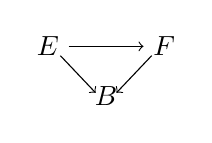
\begin{tikzpicture}[x=1.5em,y=1.2em]
  \node (E) at (0,1) {$E$};
  \node (F) at (2.8,1) {$F$};
  \node (B) at (1.4,-0.5) {$B$};
  \draw[->] (E) -- (F);
  \draw[->] (0.3,0.72) -- (1.15,-0.4);
  \draw[->] (2.5,0.72) -- (1.65,-0.4);
\end{tikzpicture}
\end{center}
\item 2-\trCell{}是 $\hcat{\mathcal{K}}$ 中如下所示的 2-\trCell $\alpha$
\begin{center}
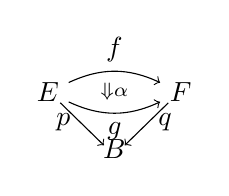
\begin{tikzpicture}[x=1.5em,y=1.2em]
  \node (E) at (0,1) {$E$};
  \node (F) at (3.2,1) {$F$};
  \node (B) at (1.6,-0.7) {$B$};
  \draw[->] (E) to[bend left=25] node[above]{$f$} (F);
  \draw[->] (E) to[bend right=25] node[below]{$g$} (F);
  \node at (1.6,1.02) {$\scriptstyle\Downarrow\alpha$};
  \draw[->] (0.3,0.68) -- (1.35,-0.6) node[pos=0.45,left]{$p$};
  \draw[->] (2.9,0.68) -- (1.85,-0.6) node[pos=0.45,right]{$q$};
\end{tikzpicture}
\end{center}
它按 $q\alpha=\mathrm{id}_p$ 的意义位于 $B$ 之上。
\end{itemize}
论证：切片\trInfinityCosmos{}的\trHomotopyTwoCategory $\hcat{(\mathcal{K}_{/B})}$
具有相同的底 1-\trCategory{}但不同的 2-\trCell{}。
这些 2-\trCell{}与 $\hcat{\mathcal{K}_{/B}}$ 的 2-\trCell{}该如何比较？
\end{exercise}
